\section{Гетероструктура}
Гетероструктура~--- полупроводниковая структура с несколькими гетеропереходами (ГП). 

Гетеропереход~--- контакт двух различных по химическому составу монокристаллических или аморфных полупроводников.

Необходимое условие образование ГП~--- совпадающие постоянные кристаллических решетки, образующими монолитный, однородный в контакте, кристалл.
Наиболее распространенные полупроводники для построения ГС:
\begin{enumerate}
  \item $GaAs$--$AlAs$;
  \item $GaN$--$AlN$;
  \item $GaSb$--$AlSb$--$InAs$;
  \item $GaAs$--$Ge$.
\end{enumerate}

\subsection{Зонная диаграмма гетероперехода}
Зонная диаграмма позволяет наглядно сранивать два и более различных полупроводника и на основе правила Андерсона получать приближенный вид зонной структуры ГП и ГС. На рис.~\ref{fig:Anderson} показан вид двух разлиных полупроводников до и после контакта \cite{Usanov}.

\begin{figure}[h]
	\centering
	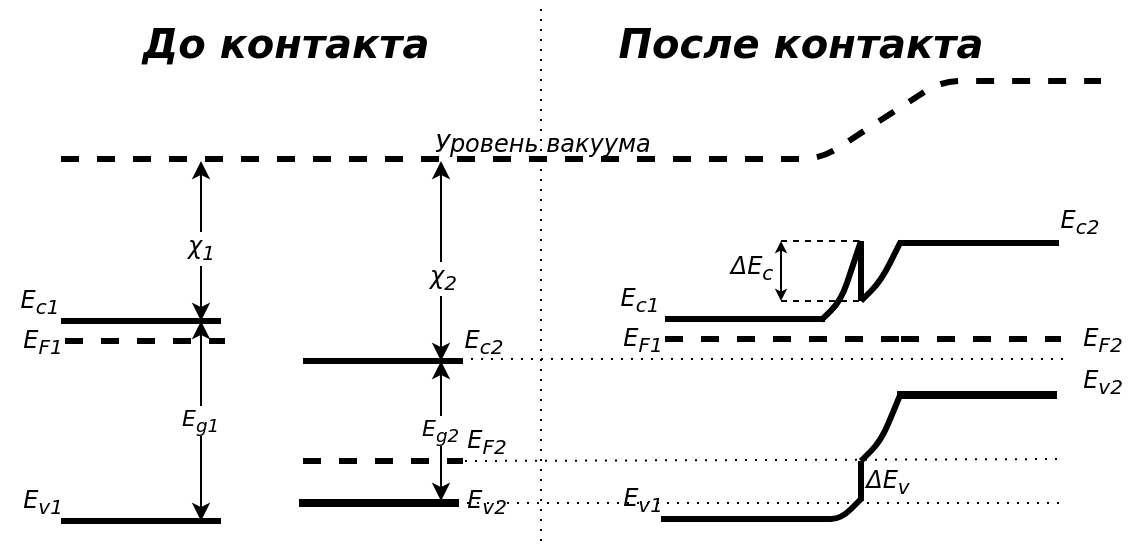
\includegraphics[width=.9\linewidth]{assets/HJ}
	\caption{Зонная диаграмма п/п до и после контакт}
	\label{fig:zone}
\end{figure}

Правило Андресона: необходимо отсчитать в сторону уменьшения от нулевой энергии свободного электрона в вакууме интервалы энергии, равные сродству соединяемых материалов к электрону, эти уровни дадут положения дна зоны проводимости.

Правило Андерсона является хорошим приближением. Для точного построения профиля зонной структуры необходимо совместное решение системы уравнений Шредингера-Пуассона.
% \subsection{Уравнение Пуассона-Больцмана}


\subsection{Резонансно--туннельная гетероструктура}
Резонансно--туннельная гетероструктура (РТГС) --- это ГС, токоперенос в которой осуществляется благодаря эффекту резонансного туннелирования \cite{Usanov}, \cite{Moskaluk}.

РТГС является ярким примером прибора, использующего эффект размерного квантования. Барьеры и ямы на рис.~\ref{img:rtgs} образуют потенциальную яму, в которой электронный газ имеет дискретные уровни энергии по одной координате, и как следствие становится 2D электронным газом.

Структурные части РГТС (рис.~\ref{img:rtgs}):
\begin{enumerate}
  \item Омический контакт;
  \item Приконтактная область;
  \item Барьер;
  \item Яма;
  \item Резервуар.
\end{enumerate}

\begin{figure}[h]
  \centering
  \includegraphics[width=.6\linewidth]{assets/rtgs}
  \caption{Структурная схема устройства с РТГС}
  \label{img:rtgs}
\end{figure}

Омический контакт выполняет роль связи РТГС с электрической схемой. Величина сопротивления искажает форму ВАХ РТГС, чем оно меньше, тем лучше.

Приконтактная область снабжает РТГС основными носителями заряда. Область сильно легируется основными носителями заряда до вырожденного состояния. Размеры приконтактных областей побираются так, чтобы концентрация основных носителей заряда приходила к равновесной на их концах.

Спейсеры изготавливаются из чистого полупроводника и предохраняют барьер и яму от проникновения туда легирующей примеси, так же спейсер препятствует накоплению заряда вблизи и внутри ямы.

Барьеры и яма формируют 2D ЭГ. Величина барьера и ямы влияют на положение резонансного уровня, прозрачность РТГС и т.д.

\subsection{Резонансно--туннельная гетероструктура на основе $Al_{x}Ga_{1-x}As$}
РГТС на основе $Al_{x}Ga_{1-x}As$ показана на рис.\ref{img:rtgsAlGaAs}. Роль барьеров в данной структуре выполняет тверндый раствор $Al$ в $GaAs$. $Al_{x}Ga_{1-x}As$ и $GaAs$ имеют различные ширины ЗЗ и сродство к электрону (табл.\ref{tab:AlGaAs}). Согласно правилу Андерсона, рельеф дна ЗП будет выглядеть, как показано на рис.~\ref{img:DifCloseAlGaAs}.

\begin{figure}[h]
  \centering
  \includegraphics[width=0.99\linewidth]{assets/rtgsAlGaAs}
  \caption{Структурная схема устройства с РТГС на основе $Al_{x}Ga_{1-x}As$}
  \label{img:rtgsAlGaAs}
\end{figure}

Потенциальная яма образуется между барьерами $Al_{x}Ga{1-x}As$. В ней элетроны имеют состояние 2D--свободного элетронного газа. Именно за счет дискретных уровней в ПЯ будет происходить токоперенос.
\begin{figure}[h]
  \centering
  \includegraphics[width=0.99\linewidth]{assets/DifCloseAlGaAs}
  \caption{Зонная структура РТГС на основе $Al_{x}Ga_{1-x}As$}
  \label{img:DifCloseAlGaAs}
\end{figure}


% \section{Гетероструктура}
% Гетероструктура~--- полупроводниковая структура с несколькими гетеропереходами (ГП). 

% ГС получили широкое распространение из-за возможности, изменяя на границах ГС ширину запрещённой зоны, управлять движением носителей заряда.

% Гетеропереход~--- контакт двух различных по химическому составу монокристаллических или аморфных полупроводников.

% ГП может образоваться между полупроводниками с абсолютно одинаковыми постоянными решетки, образующими монолитный, однородный в контакте, кристалл.
% \begin{enumerate}
% 	\item $GaAs$--$AlAs$;
% 	\item $GaN$--$AlN$;
% 	\item $GaSb$--$AlSb$--$InAs$;
% 	\item $GaAs$--$Ge$.
% \end{enumerate}

% \subsection{Зонная диаграмма гетероперехода}
% Для построения зонной диаграммы необходимо знать ширину запрещенной зоны ($E_{g}$) и положение уровня Ферми ($E_{F}$) для контактируемых полупроводников.

% \begin{figure}[h]
%   \centering
%   \includegraphics[width=.5\linewidth]{assets/Eg}
%   \caption{Зонная диаграмма перехода между полупроводниками с различными $E_{g}$}
%   \label{img:2.0.0}
% \end{figure}

% Одна из самых распространенных ГС~--- это ГС на основе твердого раствора $Al_{x}Ga_{1−x}As$, где $x$ -- это доля замещения.
% Основные характеристики $Al_{x}Ga_{1−x}As$:

% \begin{center}
  % \begin{longtable}{|c|c|}
  %   \caption{Основные параметры $Al_{x}Ga_{1−x}As$}
  %   \label{tab:2.0.0}
  %   \\ \hline
  %   Параметр & $Al_{x}Ga_{1−x}As$ \\
  %   \hline \endfirsthead
  %   \subcaption{Продолжение таблицы~\ref{tab:2.0.0}}
  %   \\ \hline \endhead
  %   \hline \subcaption{Продолжение на след. стр.}
  %   \endfoot
  %   \hline \endlastfoot
% 	Кристаллическая структура& Типа цинковой обманки \\ \hline
% 	Постоянная решетки $a[nm]$  & $0.56533+0.00078x$ \\ \hline
% 	$E_{g}^{\Gamma}[eV],\, x < 0.45$    & $1.424+1.247x$ \\ \hline
% 	$E_{g}^{\Gamma}[eV],\, x > 0.45$    & $1.656+0.215x+0.143x^{2}$ \\ \hline
% 	% $\Delta E_{c}^{\Gamma}[eV],\, x < 0.45$    & $0.773x$ \\ \hline
% 	% $\Delta E_{c}^{\Gamma}[eV],\, x > 0.45$    & $0.232-0.259x+1.147x^{2}$ \\ \hline
% 	$m_{e}^{\Gamma}$    & $0.067+0.083x$ \\ \hline
% 	$m_{lh}$    & $0.082+0.071x$ \\ \hline
% 	$N_{atoms}[1/sm^{-3}]$    & $(4.42-0.17x)10^{22}$
%   \end{longtable}
% \end{center}

% Следует также принимать во внимание, что полупроводники могут иметь минимумы зоны проводимости в разных точках зоны Брюллиена. К примеру, минимум зоны проводимости $GaAs$ находится в точке $\Gamma$, в то время как наименьший минимум в $AlAs$ близок к точке $X$. Таким образом, природа низшего минимума зоны проводимости меняется при изменении доли $Al$ в твердом растворе $Al_{x}Ga_{1−x}As$. Низший минимум в $Al_{x}Ga_{1−x}As$ изменяется от прямого расположения (минимум в $\Gamma$) зон до непрямой зонной структуры (минимум в $Х$) при содержании $Al \approx 45\%$. Обычно твердый раствор $Al_{x}Ga_{1−x}As$ получают с долей $Al$, меньше $0.45$, чтобы получить прямое расположение зон.